% COS30049 Assignment 2 report -- Bitcoin Address Activity Explorer (data and machine learning).
% Group HCMC_COS30049.1_4. Build from the repository root:
%   python tools/report_build.py        (numbers and tables from reports/tables, word count, pdflatex x3)
% Every number in the text is a \V{key} macro filled from reports/tables/*.csv or a dataset manifest by
% tools/report_numbers.py, so the prose cannot drift from the results.
\documentclass[a4paper,11pt]{article}

% ---------------------------------------------------------------- page and fonts
\usepackage[margin=2.3cm]{geometry}
\usepackage[T1]{fontenc}
\usepackage[utf8]{inputenc}
\usepackage{lmodern}
\usepackage{microtype}
\usepackage{parskip}

% ---------------------------------------------------------------- tables
\usepackage{array}
\usepackage{booktabs}
\usepackage{tabularx}
\usepackage{longtable}
\usepackage{multirow}
\renewcommand{\arraystretch}{1.18}
\newcolumntype{L}[1]{>{\raggedright\arraybackslash}p{#1}}
\newcolumntype{Y}{>{\raggedright\arraybackslash}X}
\newcolumntype{R}{>{\raggedleft\arraybackslash}X}

% ---------------------------------------------------------------- figures
\usepackage{graphicx}
\graphicspath{{../reports/figures/}}
\usepackage{float}
% let a text page carry more floats, so tables do not drift to pages of their own
\renewcommand{\topfraction}{0.9}\renewcommand{\bottomfraction}{0.8}\renewcommand{\textfraction}{0.07}
\renewcommand{\floatpagefraction}{0.75}\setcounter{totalnumber}{5}\setcounter{topnumber}{3}
\usepackage{caption}
\usepackage{subcaption}
\captionsetup{font=small, labelfont=bf}
\captionsetup[table]{position=top}
\usepackage{tikz}
\usetikzlibrary{arrows.meta, positioning, fit, backgrounds}

% ---------------------------------------------------------------- text
\usepackage{amsmath}
\usepackage{enumitem}
\setlist{nosep, leftmargin=1.4em}
\usepackage{xcolor}

% \V{key}: a number written by tools/report_numbers.py; an unknown key stops the build.
\newcommand{\V}[1]{\ifcsname v@#1\endcsname\csname v@#1\endcsname\else
  \PackageError{report}{Unknown number key #1}{Run python tools/report_numbers.py}\fi}
% Written by tools/report_numbers.py from reports/tables and the manifests. Do not edit.
\expandafter\def\csname v@abl.refined_flag_rate\endcsname{10.4\%}
\expandafter\def\csname v@abl.refined_recall\endcsname{0.655}
\expandafter\def\csname v@abl.written_flag_rate\endcsname{31.3\%}
\expandafter\def\csname v@abl.written_recall\endcsname{0.439}
\expandafter\def\csname v@act.ds10_gap\endcsname{13.1}
\expandafter\def\csname v@act.ds1_gap\endcsname{23.1}
\expandafter\def\csname v@agree.base_range\endcsname{0.24--0.37}
\expandafter\def\csname v@agree.base_txgpt\endcsname{0.06}
\expandafter\def\csname v@cls.ell_rf_f1\endcsname{0.815}
\expandafter\def\csname v@cls.ell_rf_f1_ci\endcsname{[0.796, 0.835]}
\expandafter\def\csname v@cls.heist_temporal_max_f1\endcsname{0.07}
\expandafter\def\csname v@cls.lofo_range\endcsname{0.3\%--3.3\%}
\expandafter\def\csname v@conf.after\endcsname{87.5\%}
\expandafter\def\csname v@conf.before\endcsname{78.4\%}
\expandafter\def\csname v@conf.nominal\endcsname{90\%}
\expandafter\def\csname v@ds1.baseline.burst_event\endcsname{0.776}
\expandafter\def\csname v@ds1.baseline.burst_tx\endcsname{0.381}
\expandafter\def\csname v@ds1.baseline.flag_rate\endcsname{10.4\%}
\expandafter\def\csname v@ds1.baseline.mean\endcsname{0.655}
\expandafter\def\csname v@ds1.baseline.precision\endcsname{0.125}
\expandafter\def\csname v@ds1.blocks\endcsname{20}
\expandafter\def\csname v@ds1.candidates\endcsname{5{,}995}
\expandafter\def\csname v@ds1.fusion.flag_rate\endcsname{9.4\%}
\expandafter\def\csname v@ds1.fusion.mean\endcsname{0.682}
\expandafter\def\csname v@ds1.fusion.precision\endcsname{0.161}
\expandafter\def\csname v@ds1.main\endcsname{25}
\expandafter\def\csname v@ds1.main_max_tx\endcsname{1{,}000}
\expandafter\def\csname v@ds1.main_min_days\endcsname{90}
\expandafter\def\csname v@ds1.main_min_tx\endcsname{50}
\expandafter\def\csname v@ds1.short\endcsname{3}
\expandafter\def\csname v@ds1.short_max_tx\endcsname{9}
\expandafter\def\csname v@ds1.short_min_tx\endcsname{3}
\expandafter\def\csname v@ds1.tx\endcsname{7{,}966}
\expandafter\def\csname v@ds1.txgpt.flag_rate\endcsname{1.5\%}
\expandafter\def\csname v@ds1.txgpt.mean\endcsname{0.547}
\expandafter\def\csname v@ds1.txgpt.precision\endcsname{0.421}
\expandafter\def\csname v@ds10.baseline.ci\endcsname{[0.334, 0.528]}
\expandafter\def\csname v@ds10.baseline.mean\endcsname{0.431}
\expandafter\def\csname v@ds10.fusion.ci\endcsname{[0.279, 0.473]}
\expandafter\def\csname v@ds10.fusion.mean\endcsname{0.367}
\expandafter\def\csname v@ds10.rows\endcsname{5{,}785}
\expandafter\def\csname v@ds10.sample_blocks\endcsname{6}
\expandafter\def\csname v@ds10.short\endcsname{3}
\expandafter\def\csname v@ds10.tier_quota\endcsname{8}
\expandafter\def\csname v@ds10.txgpt.ci\endcsname{[0.534, 0.657]}
\expandafter\def\csname v@ds10.txgpt.mean\endcsname{0.598}
\expandafter\def\csname v@ds2.blocks\endcsname{200}
\expandafter\def\csname v@ds2.check_addresses\endcsname{2{,}933}
\expandafter\def\csname v@ds2.ds1_removed\endcsname{1{,}533}
\expandafter\def\csname v@ds2.fetch_errors\endcsname{106}
\expandafter\def\csname v@ds2.kept\endcsname{4{,}012}
\expandafter\def\csname v@ds2.rows\endcsname{898{,}490}
\expandafter\def\csname v@ds2.too_few\endcsname{4{,}422}
\expandafter\def\csname v@ds2.too_many\endcsname{539}
\expandafter\def\csname v@ds2.visited\endcsname{9{,}079}
\expandafter\def\csname v@eda.core_share\endcsname{60.5\%}
\expandafter\def\csname v@eda.dir_differ\endcsname{9}
\expandafter\def\csname v@eda.dir_tested\endcsname{23}
\expandafter\def\csname v@eda.ell_test_share\endcsname{6.5\%}
\expandafter\def\csname v@eda.ell_train_share\endcsname{11.6\%}
\expandafter\def\csname v@eda.ell_unknown\endcsname{77\%}
\expandafter\def\csname v@eda.f1_skew_log\endcsname{$-$0.44}
\expandafter\def\csname v@eda.f1_skew_raw\endcsname{38.9}
\expandafter\def\csname v@eda.f4_kurt_raw\endcsname{7{,}813}
\expandafter\def\csname v@eda.heist_max_effect\endcsname{0.13}
\expandafter\def\csname v@eda.heist_share\endcsname{1.4\%}
\expandafter\def\csname v@eda.pca_variance\endcsname{87.3\%}
\expandafter\def\csname v@eda.rho_f1f4\endcsname{0.33}
\expandafter\def\csname v@eda.rho_f2f3\endcsname{$-$0.57}
\expandafter\def\csname v@eda.scale_ratio\endcsname{9{,}949}
\expandafter\def\csname v@ell.labelled\endcsname{46{,}564}
\expandafter\def\csname v@ell.rows\endcsname{203{,}769}
\expandafter\def\csname v@heist.positives\endcsname{41{,}413}
\expandafter\def\csname v@heist.rows\endcsname{2{,}916{,}697}
\expandafter\def\csname v@inj.burst\endcsname{10}
\expandafter\def\csname v@inj.burst_hours\endcsname{24}
\expandafter\def\csname v@inj.dormant_max\endcsname{120}
\expandafter\def\csname v@inj.dormant_min\endcsname{60}
\expandafter\def\csname v@inj.per_pattern\endcsname{50}
\expandafter\def\csname v@inj.spike\endcsname{10}
\expandafter\def\csname v@label.ell_rf_lift\endcsname{12.2}
\expandafter\def\csname v@lm.full_ds10\endcsname{93.1\%}
\expandafter\def\csname v@lm.full_ds7\endcsname{96.9\%}
\expandafter\def\csname v@lm.glossary\endcsname{48\%}
\expandafter\def\csname v@lm.guard_ds10\endcsname{100.0\%}
\expandafter\def\csname v@lm.guard_ds7\endcsname{100.0\%}
\expandafter\def\csname v@lm.pooled\endcsname{94.8\%}
\expandafter\def\csname v@lm.pooled_ci\endcsname{95\% interval [94.1\%, 95.4\%]}
\expandafter\def\csname v@lm.pretrain_tokens\endcsname{5.0}
\expandafter\def\csname v@obj.reviewer\endcsname{No ratings recorded at submission; the blind sheet is in reports/reviewer}
\expandafter\def\csname v@obj.walkthrough\endcsname{No session recorded at submission; moved to the Assignment 3 usability study}
\expandafter\def\csname v@reg.gap_skill\endcsname{60\%}
\expandafter\def\csname v@reg.size_skill\endcsname{10\%}
\expandafter\def\csname v@sel.sanity\endcsname{20\%}
\expandafter\def\csname v@sel.stability_target\endcsname{0.7}
\expandafter\def\csname v@sig.fusion_p\endcsname{0.324}
\expandafter\def\csname v@stats.ds10_baseline_rank1\endcsname{96\%}
\expandafter\def\csname v@tech.tests\endcsname{273}
\expandafter\def\csname v@txgpt.s_params\endcsname{820{,}352}
\expandafter\def\csname v@txgpt.vocab\endcsname{94}
\expandafter\def\csname v@wf.baseline_range\endcsname{0.650--0.658}
\expandafter\def\csname v@wf.cutoffs\endcsname{4}
\expandafter\def\csname v@wf.lof_range\endcsname{0.331--0.410}

\newcommand{\limitation}{\emph{Unusual activity requires investigation; it does not indicate wrongdoing.}}
\newcommand{\code}[1]{\texttt{\small #1}}
% \FloatBarrier: if figures or tables are still waiting to be placed, place them before going on (a new page);
% otherwise do nothing. Keeps a section's floats out of the next section (placeins is not in TinyTeX here).
\makeatletter
\newcommand{\FloatBarrier}{\par\begingroup\let\@elt\relax
  \edef\@tempa{\@botlist\@deferlist\@dbldeferlist}%
  \ifx\@tempa\@empty\endgroup\else\endgroup\clearpage\fi}
\makeatother

% numbered reference list [1]-[N], alphabetical, hanging indent (as in Assignment 1)
\newcounter{refnum}
\newenvironment{references}{%
  \sloppy\begin{list}{[\arabic{refnum}]}{\usecounter{refnum}\setlength{\labelwidth}{2.2em}%
    \setlength{\leftmargin}{2.8em}\setlength{\labelsep}{0.6em}%
    \setlength{\itemsep}{0.35\baselineskip}\setlength{\parsep}{0pt}}\small}%
  {\end{list}}

% ---------------------------------------------------------------- links (last)
\usepackage[hyphens]{url}
\usepackage[colorlinks=true, linkcolor=blue!50!black, citecolor=blue!50!black,
            urlcolor=blue!60!black]{hyperref}
\hypersetup{pdftitle={Bitcoin Address Activity Explorer: Detecting Unusual Transactions with Machine Learning},
            pdfauthor={HCMC\_COS30049.1\_4}}

\begin{document}

% Cover page (not counted). The brief asks for the title, the group name and ID, every student's name and ID,
% and the tutor's name.
\begin{titlepage}
\centering
\vspace*{2.2cm}
{\Large COS30049 Computing Technology Innovation Project\par}
\vspace{0.4cm}
{\large Assignment 2: Data Processing and Machine Learning\par}
\vspace{1.6cm}
{\huge\bfseries Bitcoin Address Activity Explorer\par}
\vspace{0.3cm}
{\Large Detecting Unusual Transactions with Machine Learning\par}
\vspace{1.8cm}

\begin{tabular}{@{}ll@{}}
\toprule
Group & HCMC\_COS30049.1\_4 (Group 4) \\
Tutor & Arthur Hoang \\
\midrule
Cam Dan Bui & 105967074 \\
Cao Tri Tran & 106214726 \\
Le Quang Anh Hoang & 106218605 \\
Minh Khang Nguyen & 106216803 \\
\bottomrule
\end{tabular}

\vspace{1.6cm}
Swinburne University of Technology, Ho Chi Minh City campus\par
Submitted 7 November 2026\par
\vfill
{\small Word count: 2{,}871 words in the body (Sections 1--8), counted by
\code{tools/report\_wordcount.py}; tables, captions, the cover, contents, references and appendix are excluded.\par}
\end{titlepage}


\pagenumbering{roman}
\tableofcontents
\clearpage
\pagenumbering{arabic}

% Body: the brief's sections in the brief's order (counted towards the 3,000 words).
\section{Introduction}
\label{sec:intro}

Banks, exchanges and payment providers that handle cryptocurrency must decide which of many transactions deserve
a closer look, the topic the brief calls cybersecurity threat detection in banking. A Bitcoin address's history is
public, but a block explorer shows it only as a long, unexplained list.

Our project, the Bitcoin Address Activity Explorer, ranks every transaction of an address by how \emph{unusual}
it is \emph{for that address's own past} and says why in plain words. Its intended user is a student researcher
or analyst examining one address who needs to know where to look first. It is an investigation aid, never a
verdict: every flag carries the line \limitation

This report covers Assignment~2: the data we collected and processed, the analysis that shaped the features,
the models we trained and why we chose them, and their evaluation. Every model was trained by our team, and
both language models were trained from scratch. The prediction interface that Assignment~3's web application
will call is ready.

\section{Problem Framing}
\label{sec:problem}

\textbf{The challenge.} We must decide which transactions deserve attention when no labels exist, and explain
each decision, because the user acts on the reason, not on a score.

\textbf{Limits of existing solutions.} Block explorers list transactions without ranking them. A fixed rule, such
as ``flag anything above one bitcoin'', ignores scale: wallets, trading bots and cold storage behave very
differently, and the median amounts of our addresses differ by a factor of \V{eda.scale_ratio}. One threshold
over-flags busy addresses, misses changes on quiet ones, and cannot follow changing behaviour. Supervised models
trained on public labelled datasets learn from sparse labels and from aggregated or anonymised features that cannot
be computed for an arbitrary address (Akcora et al.\ 2020; Elmougy and Liu 2023), and their accuracy collapses when
behaviour changes (Pareja et al.\ 2020).

\textbf{Why machine learning.} Learning can model each address's normal behaviour, find structure without
labels, read a history as a sequence, and use labels where they exist (Hilal, Gadsden and Yawney 2022; Han et
al.\ 2022). Real transactions have no target label, so we combine unsupervised methods with regression and use
classification only on labelled data. Four research questions guide the work:
\begin{enumerate}[label=RQ\arabic*]
  \item Which stable method best finds transactions planted in an address's own history?
  \item How well do classifiers perform on labelled data over time and on unseen families?
  \item Does ``unusual'' coincide with the labelled datasets' own illicit class?
  \item Does a sequence model trained on other addresses generalise better than per-address statistics, and can a
    language model trained from scratch explain flags faithfully?
\end{enumerate}

\section{Data Collection}
\label{sec:collection}

Table~\ref{tab:datasets} lists the eight datasets: three collections of public blockchain data of our own, two
public labelled datasets, and three text corpora for the language models.

\begin{table}[htbp]
\centering
\footnotesize
\caption{The datasets and the role of each (tx: transactions).}
\label{tab:datasets}
\begin{tabularx}{\textwidth}{@{}l L{3.0cm} L{3.7cm} L{3.0cm} Y@{}}
\toprule
ID & Dataset & Source (licence) & Size & Role \\
\midrule
DS1 & Our Esplora snapshot & Blockstream Esplora API (public data) & 25\,+\,3 addresses, 7{,}966 tx & Every scoring method; evaluation \\
DS2 & Our Esplora crawl (hashed IDs) & Esplora API via mempool.space & 4{,}012 addresses, 898{,}490 tx & Trains TxGPT; check on unseen addresses \\
DS3 & Elliptic data set & Kaggle (CC BY-NC-ND 4.0) & 203{,}769 tx & Classification \\
DS4 & BitcoinHeist & UCI repository 526 (CC BY 4.0) & 2{,}916{,}697 address-days & Classification \\
DS5 & FineWeb-Edu & Hugging Face (ODC-By 1.0) & 5.0 billion tokens used & Assistant pretraining \\
DS6 & smol-smoltalk & Hugging Face (Apache 2.0) & chat conversations & Assistant chat stage \\
DS7 & Our explanation pairs & Built from DS1 and DS2 facts & question--answer pairs & Teaching and testing the Assistant \\
DS10 & A teammate's snapshot & Esplora API, refetched and cross-checked & 27 addresses, 5{,}785 tx & Held-out final test of every model \\
\bottomrule
\end{tabularx}
\end{table}


\subsection{Our own collections: DS1, DS2 and DS10}

Assignment~1 chose Blockstream's Esplora API (Blockstream n.d.) because it returns each address's confirmed
history with every transaction's inputs and outputs. The DS1 selection rule was recorded, with its random seed, before any address was fetched: take
\V{ds1.blocks} block heights from the previous four weeks, gather their output addresses (\V{ds1.candidates}
candidates), shuffle them and visit them in order. A \emph{main} address needs
\V{ds1.main_min_tx}--\V{ds1.main_max_tx} confirmed transactions over at least \V{ds1.main_min_days} days; a
\emph{short-history} address needs \V{ds1.short_min_tx}--\V{ds1.short_max_tx}, so the Explorer's ``not enough
history'' state is tested too. An address is kept only if its transaction count matches the API's own count,
its received and sent sums match the API's totals, and no transaction is duplicated or unconfirmed. DS1 holds
\V{ds1.main} main and \V{ds1.short} short addresses with \V{ds1.tx} transactions.

DS2 applies the same client to \V{ds2.blocks} blocks spread over twelve months, after removing every address in
DS1's candidate pool (\V{ds2.ds1_removed}) so that DS1 never leaks into TxGPT's training data. Of
\V{ds2.visited} addresses visited, \V{ds2.kept} were kept; they are stored only as salted hashes. DS10 is a
teammate's independent snapshot, collected with their own script and rule. We refetched it with our client: all
\V{ds10.rows} transactions agree with the teammate's file, and no address is shared with DS1 or DS2.

\subsection{Public labelled data and text corpora}

Elliptic (DS3) labels \V{ell.labelled} of its \V{ell.rows} transactions as illicit or licit, its own class
names, over 49 time steps (Elmougy and Liu 2023). BitcoinHeist (DS4) has \V{heist.rows} address-days, of which
\V{heist.positives} belong to ransomware families (Akcora et al.\ 2020; UCI Machine Learning Repository 2020).
Elliptic's licence allows no derivatives, so we ship a download script instead of processed data. The Assistant
learned English from FineWeb-Edu (DS5; Penedo et al.\ 2024), conversation from smol-smoltalk (DS6; Ben Allal et
al.\ 2025), and explanations from DS7, question--answer pairs built from our own pipeline's facts.

\subsection{Challenges and how we addressed them}

\begin{itemize}
  \item \textbf{Rate limits.} The public API allows about 700 requests an hour. Our client paces requests, backs
    off on refusals, falls back to the compatible mempool.space API (mempool.space n.d.), caches every raw reply
    and resumes after interruptions; \V{ds2.fetch_errors} addresses that failed every retry were logged and
    skipped.
  \item \textbf{Selection bias.} \V{ds2.too_many} visited addresses exceeded the transaction cap (typically busy
    services) and \V{ds2.too_few} had too little history. Sampling recent blocks favours active addresses, and
    an address is not a person; we state these limits rather than hide them.
  \item \textbf{No ground truth.} Real transactions carry no labels, so we evaluate on transactions we plant
    (Section~\ref{sec:processing}) and use labelled metrics only on DS3 and DS4.
\end{itemize}

\section{Data Processing}
\label{sec:processing}

Figure~\ref{fig:pipeline} shows the pipeline; each step is one module of our \code{explorer} package.

\begin{figure}[ht]
\centering
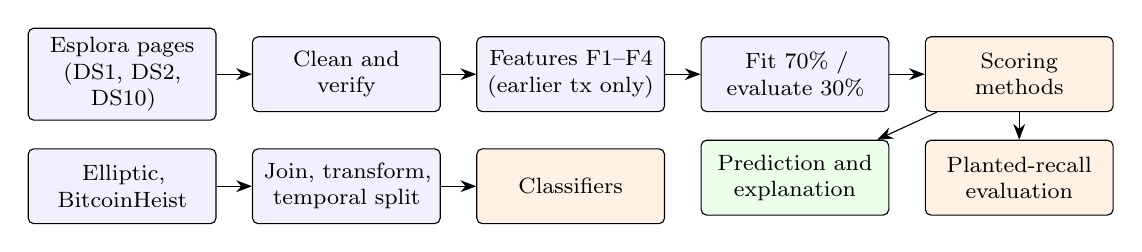
\begin{tikzpicture}[node distance=0.35cm and 0.45cm, font=\footnotesize,
  box/.style={draw, rounded corners=2pt, align=center, minimum height=0.95cm, text width=2.15cm, fill=#1},
  box/.default=blue!6, >={Stealth[length=2mm]}]
  \node[box] (raw) {Esplora pages\\(DS1, DS2, DS10)};
  \node[box, right=of raw] (clean) {Clean and\\verify};
  \node[box, right=of clean] (feat) {Features F1--F4\\(earlier tx only)};
  \node[box, right=of feat] (split) {Fit 70\% /\\evaluate 30\%};
  \node[box=orange!10, right=of split] (models) {Scoring\\methods};
  \node[box=orange!10, below=of models] (eval) {Planted-recall\\evaluation};
  \node[box=green!8, left=of eval] (pred) {Prediction and\\explanation};
  \node[box, below=of raw] (lab) {Elliptic,\\BitcoinHeist};
  \node[box, right=of lab] (labp) {Join, transform,\\temporal split};
  \node[box=orange!10, right=of labp] (cls) {Classifiers};
  \draw[->] (raw) -- (clean); \draw[->] (clean) -- (feat); \draw[->] (feat) -- (split);
  \draw[->] (split) -- (models); \draw[->] (models) -- (eval); \draw[->] (models) -- (pred);
  \draw[->] (lab) -- (labp); \draw[->] (labp) -- (cls);
\end{tikzpicture}
\caption{The processing pipeline. Our Bitcoin data (top) feeds the scoring methods; the labelled datasets
(bottom) feed the classifiers. The two paths never mix.}
\label{fig:pipeline}
\end{figure}

\textbf{Cleaning and missing values.} DS1 passes five checks: parse every saved page, keep confirmed
transactions, remove duplicate (address, transaction) pairs, drop transactions that neither pay nor spend from
the address, and sort by time. None removed a row, because the collection checks had already rejected faulty
histories. The source data has no missing values; features are empty by design when an address has too little
history, and such transactions are shown as ``not scored'' rather than imputed.

\textbf{Feature engineering.} For each transaction we compute the address's net amount (received minus sent) and
direction, then the four features of Table~\ref{tab:features}. Each is compared with the same address's history
using a robust z-score: the distance from the median in units of the median absolute deviation, which one
extreme past value cannot distort (Blázquez-García et al.\ 2022). Heavy-tailed features are compared on a
logarithmic scale, and the spread has a floor so that a run of identical values cannot divide by zero. This is
the normalisation: every score is relative to the address itself.

\begin{table}[htbp]
\centering
\small
\caption{The four explained features (A1, refined). Each becomes a robust z-score against the same address's earlier history.}
\label{tab:features}
\begin{tabularx}{\textwidth}{@{}l l Y l@{}}
\toprule
ID & Name & Definition & Compared on \\
\midrule
F1 & Size & Amount the address received or sent (BTC) & log10; same direction only \\
F2 & Burst & Earlier transactions in the previous 7 days & raw count \\
F3 & Gap & Hours since the address's previous transaction & log10 \\
F4 & Relative size & Amount divided by the usual amount in the same direction & log10 \\
\bottomrule
\end{tabularx}
\par\smallskip\parbox{\textwidth}{\footnotesize Each feature is compared with earlier transactions of the same address in the previous 30 days, extended back to reach 20; a transaction is scored once the address has at least 10 earlier transactions over 14 days.}
\end{table}


\textbf{Time safety.} A transaction's features use only \emph{strictly earlier} transactions of the same address,
and transactions in the same block are never each other's history. Models fit on each address's earlier 70\% and
are evaluated on the rest, and every scaler sits inside a scikit-learn pipeline fitted on training rows only.
These rules prevent leakage (Kapoor and Narayanan 2023).

\textbf{Planted transactions.} To measure detection without labels we plant three patterns into copies of each
history's evaluation period (Lai et al.\ 2021): a \emph{spike} of \V{inj.spike}$\times$ the address's usual amount,
a \emph{burst} of \V{inj.burst} transactions within \V{inj.burst_hours} hours, and a \emph{dormant} address waking
after \V{inj.dormant_min}--\V{inj.dormant_max} days. Each seed plants \V{inj.per_pattern} of each pattern. Tuning
seeds never produce reported results.

\textbf{Labelled datasets.} Elliptic's features and classes are joined on the transaction identifier and split by
time (steps 1--34 to train and validate, 35--49 to test), with all features (AF) or local ones (LF). In
BitcoinHeist every ransomware family becomes the positive class, the five heavy-tailed features are log
transformed, and \code{year}, \code{day} and \code{address} are excluded as features because they would leak the
split or identify the row.

\textbf{Language-model inputs.} TxGPT writes each transaction as six tokens (gap, direction, amount, inputs,
outputs, fee rate) from a vocabulary of \V{txgpt.vocab}. DS7 pairs a question about one transaction with its facts
and the template's answer, split by address so that no address spans two splits.

\section{Data Analysis}
\label{sec:analysis}

The analysis lives in \code{notebooks/01\_eda.ipynb}, and every statistic below is written to
\code{eda\_tests.csv}. Each finding is stated as an observation, the statistic behind it, and the decision it
informed.

\textbf{Finding 1: the features are heavy-tailed.} Amounts, gaps and ratios span several orders of magnitude
(Figure~\ref{fig:distributions}). The raw amount has a skewness of \V{eda.f1_skew_raw}, but only
\V{eda.f1_skew_log} on a logarithmic scale; the size ratio's excess kurtosis is \V{eda.f4_kurt_raw}. A mean and
standard deviation would be dominated by a few extreme values, so we compare on log scales and use the median
and median absolute deviation.

\begin{figure}[ht]
\centering
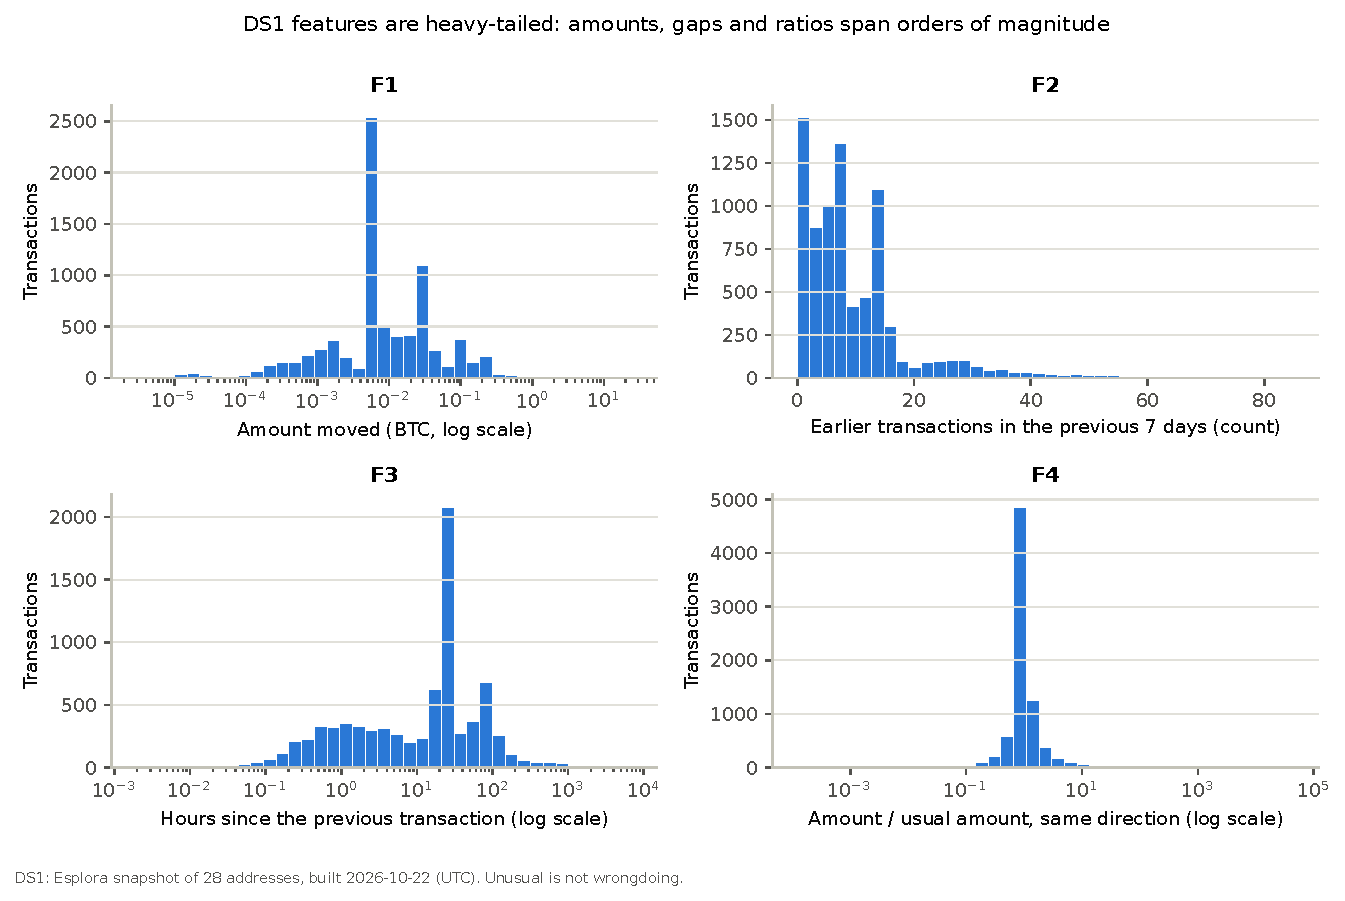
\includegraphics[width=0.82\textwidth]{eda_feature_distributions.pdf}
\caption{DS1's four features. Amounts (F1), gaps (F3) and size ratios (F4) span orders of magnitude, which is why
they are compared on log scales with robust statistics.}
\label{fig:distributions}
\end{figure}

\textbf{Finding 2: every address has its own scale.} The median amounts of DS1's main addresses differ by a
factor of \V{eda.scale_ratio}, and for \V{eda.dir_differ} of the \V{eda.dir_tested} addresses with enough
transactions in both directions, received and sent amounts differ (Mann--Whitney U, $p<0.05$;
Figure~\ref{fig:direction}). One global threshold cannot fit every address, so each feature is compared with the
same address's history and amounts only with earlier transactions in the same direction. The ablation confirms
the decision: A1's original definition, without these refinements, flags \V{abl.written_flag_rate} of real
transactions with a mean planted recall of \V{abl.written_recall}, against \V{abl.refined_flag_rate} and
\V{abl.refined_recall} for the refined features (\code{eval\_ablation.csv}).

\begin{figure}[ht]
\centering
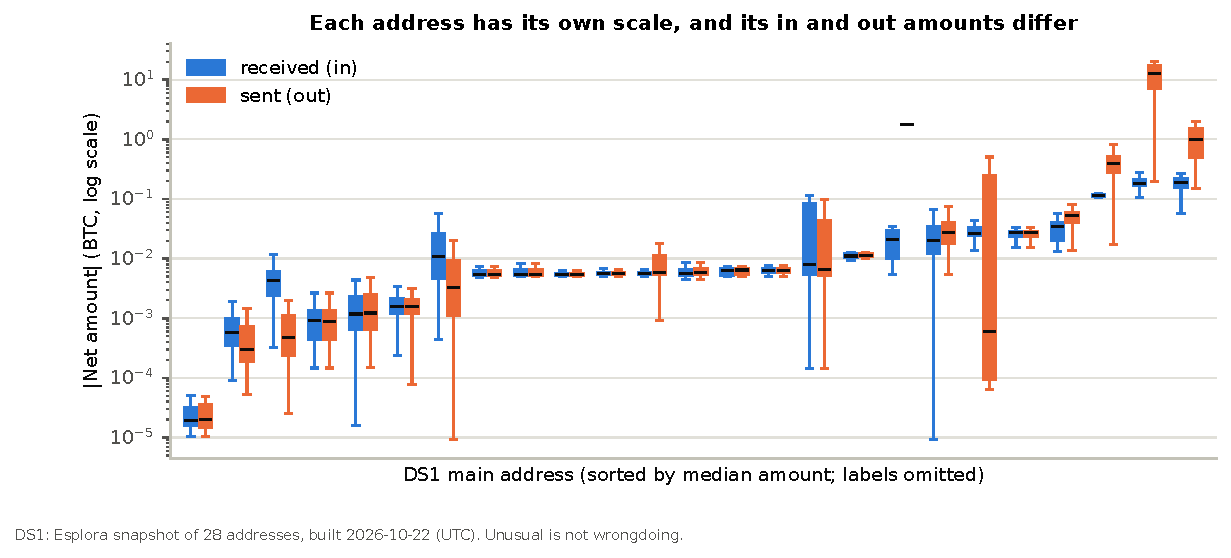
\includegraphics[width=0.9\textwidth]{eda_direction_amounts.pdf}
\caption{Received and sent amounts per DS1 main address (box: quartiles; line: median). Scales differ by four
orders of magnitude, and many addresses send amounts unlike those they receive.}
\label{fig:direction}
\end{figure}

\textbf{Finding 3: labels are rare and drift over time.} Elliptic's illicit share among labelled transactions is
\V{eda.ell_train_share} in the training steps but \V{eda.ell_test_share} in the test steps, and
\V{eda.ell_unknown} of all rows are unlabelled. BitcoinHeist's positives are \V{eda.heist_share} of rows, and
every feature separates them only weakly (largest rank-biserial effect \V{eda.heist_max_effect}). Accuracy
would reward predicting the majority class (Chicco and Jurman 2020), so we split by time, report precision,
recall, F1 and the area under the precision--recall curve (PR-AUC), and include class weights in tuning. The weak
BitcoinHeist effects also anticipated its poor classification results in Section~\ref{sec:evaluation}.

\section{Machine Learning Model Selection}
\label{sec:selection}

\textbf{Criteria.} A scoring method for the Explorer had to (1) work without labels, (2) judge each transaction
against its own address's earlier history, (3) give a reason the user can check, (4) be stable, keeping a
top-50 overlap (Jaccard) of at least \V{sel.stability_target} across refits, (5) flag no more than
\V{sel.sanity} of any address's transactions, and (6) run on a laptop CPU.

\textbf{Candidates} (Table~\ref{tab:candidates}). No detector wins on every kind of anomaly (Han et al.\ 2022), so
each family covers a different idea of ``unusual''. The baseline flags a transaction when any feature lies far from
the address's median. Clustering scores the distance to normal transactions (Ikotun et al.\ 2023; Bushra and Yi
2021). Regression predicts each amount and gap from earlier history and scores the miss; conformal calibration
gives ranges with stated coverage (Angelopoulos and Bates 2023). Isolation Forest and the Local Outlier Factor (LOF)
are general outlier detectors (Boukerche, Zheng and Alfandi 2021). Fusion combines the regression and Isolation
Forest scores at a fixed flag budget. TxGPT, a small transformer trained from scratch on DS2, scores each
transaction by its surprisal, the negative log-probability of what happened (Le and Zhang 2022). For labelled data
we compared a linear model, a neighbour-based model and two tree ensembles, which remain strong on tabular data
(Grinsztajn, Oyallon and Varoquaux 2022).

\begin{table}[htbp]
\centering
\footnotesize
\caption{Every model trained, by family. All were tuned on data that never produced a reported result.}
\label{tab:candidates}
\begin{tabularx}{\textwidth}{@{}L{2.2cm} L{4.0cm} l L{3.4cm} Y@{}}
\toprule
Family & Models & Data & Output & Tuned \\
\midrule
Statistics & Robust z-score baseline (A1) & DS1 & Largest $|z|$ over F1--F4 & Flag threshold \\
Clustering & K-Means; DBSCAN & DS1 & Distance to normal clusters & $k$; eps, min.\ samples \\
Clustering & K-Means address profiles & DS1, DS2 & Activity profile in words & $k$ (silhouette) \\
Regression & Ridge; random forest; hist.\ gradient boosting & DS1 & Miss on predicted amount and gap & Per-model grids \\
Regression & Quantile boosting + conformal & DS1 & Distance outside a calibrated range & Quantiles, coverage \\
Outlier detection & Isolation Forest; LOF (novelty) & DS1 & Isolation depth; local density & Trees, samples; neighbours \\
Combination & Score fusion & DS1 & Weighted pair of scores & Weights at a flag budget \\
Classification & Logistic regression; KNN; random forest; hist.\ gradient boosting & DS3, DS4 & Class probability & Validation split \\
Sequence model & TxGPT (trained from scratch) & DS2 & Surprisal of each transaction & 3 sizes $\times$ 3 seeds \\
Language model & Explorer Assistant, 152M (trained from scratch) & DS5--DS7 & Explanation (guardrailed) & Adoption rule \\
\bottomrule
\end{tabularx}
\end{table}


\textbf{Tuning and preliminary tests.} Every search is in \code{tuning\_*.csv}, run on plant seeds that never score reported results. K-Means' $k$ came from the silhouette score and Davies--Bouldin index,
DBSCAN's radius from the elbow of its k-distance graph, and each regressor was compared with a naive forecast
(Table~\ref{tab:unsupervised}). Each method was then retrained in stages, and a stage was kept only if it passed a
gate fixed in advance: higher recall with a bootstrap interval above zero, and no pattern falling by more than its
seed spread. LOF, K-Means and DBSCAN passed; the other scoring and classifier stages failed and were dropped
(\code{stages.csv}).

\textbf{The selection rule}, fixed in Assignment~1, picks the stable method with the highest mean planted recall,
and within five points the easier one to explain. Fusion scored highest (\V{ds1.fusion.mean}), but the baseline
(\V{ds1.baseline.mean}) lies within the margin, and the difference is not significant (paired bootstrap,
$p=\V{sig.fusion_p}$). The Explorer therefore uses the baseline, whose reasons map directly to the features.

\textbf{Explanations.} The \emph{Explorer Assistant}, a language model, may phrase an
explanation only if it passes a code guardrail: numbers from the facts, the limitation line, no banned word, correct
comparison direction, and a verdict matching the flag. Otherwise a fixed template is shown, because language models
can state numbers absent from their input (Ji et al.\ 2023).

\section{Implementation}

\subsection{Technical implementation}
\label{sec:technical}

The project is written in Python with pandas, scikit-learn and matplotlib (The pandas
development team 2024; scikit-learn developers 2025; The Matplotlib Development Team 2025); PyTorch is used only
for the two language models (Ansel et al.\ 2024). The \code{explorer} package has three layers (data and features,
model execution, explanation), with one module per pipeline step, all run through one command-line tool;
\code{config/settings.json} holds every threshold, window, grid and seed. Versions are pinned in a conda environment, and \V{tech.tests} tests check properties such as time
safety and the guardrail. A full rebuild runs offline, and a script compares the rebuilt tables with the committed
ones number by number (Pineau et al.\ 2021).

TxGPT was trained on GPUs in three sizes with three seeds each; the sizes tie, so the smallest
(\V{txgpt.s_params} parameters) was kept. The Assistant follows a modern decoder design (Touvron et al.\ 2023) and was
pretrained on \V{lm.pretrain_tokens} billion DS5 tokens, more than the compute-optimal budget of about 20 tokens per
parameter (Hoffmann et al.\ 2022), then taught conversation (DS6) and explanations (DS7). It predicts on a CPU.

The \code{Predictor} class is the interface Assignment~3 will call. Three commands expose it: \code{predict address}
scores an address's whole timeline, \code{predict what-if} scores a hypothetical next transaction (the brief's
``user input to prediction''), and \code{predict explain} explains any transaction.

\subsection{Implementation evaluation}
\label{sec:evaluation}

\textbf{Objectives.} Table~\ref{tab:objectives} compares the results with Assignment~1's targets. The baseline meets the recall target on spikes and dormant addresses but not on bursts counted per
transaction (\V{ds1.baseline.burst_tx}), although it finds \V{ds1.baseline.burst_event} of burst events, and four
DS1 addresses break the sanity rule. We report these rather than move the targets. Two objectives that need people
outside the build remain open.

\begin{table}[htbp]
\centering
\footnotesize
\caption{Assignment~1's objectives for the selected method (the robust z baseline) and the results.}
\label{tab:objectives}
\begin{tabularx}{\textwidth}{@{}Y L{5.6cm} l@{}}
\toprule
Objective (set in Assignment~1) & Result & Status \\
\midrule
Snapshot of 20--30 main addresses (50+ tx, 90+ days) and 2--3 short ones & 25 main and 3 short addresses & Met \\
Planted recall $\geq$ 70\% for 2 of 3 patterns & Spike 0.744, dormant 0.840, burst 0.381 & Met \\
Stability: top-50 Jaccard $\geq$ 0.7 & 1.000 & Met \\
Sanity: no address over 20\% flagged & DS1: 4 addresses over; DS10: 0 & Partly met \\
Method agreement reported & Baseline--fusion Jaccard 0.512 & Met \\
Blind reviewer check (Cohen's kappa) & Pending: two teammates rate reports/reviewer/sheet.csv & Open \\
Accuracy, precision, recall, F1 where labels exist & DS3 and DS4 (Table~\ref{tab:classifiers}) & Met \\
\bottomrule
\end{tabularx}
\end{table}


\textbf{Scoring methods on DS1} (Table~\ref{tab:ds1}). Each method finds different patterns
(Figure~\ref{fig:recall}). Regression finds every planted burst event but few dormant addresses, LOF misses most
spikes, and only fusion, the baseline and TxGPT catch most spikes, burst events and dormant addresses. TxGPT flags
the fewest real transactions (\V{ds1.txgpt.flag_rate}) and so has the highest precision lower bound
(\V{ds1.txgpt.precision} against \V{ds1.baseline.precision}); a flag that is not a plant may still be worth a look,
so real-data precision can only be bounded.

\begin{table}[htbp]
\centering
\footnotesize
\caption{Scoring methods on DS1 (sorted by mean planted recall).}
\label{tab:ds1}
\begin{tabularx}{\textwidth}{@{}L{3.6cm} l r r r l r R@{}}
\toprule
Method & Family & Spike & Burst & Dormant & Mean [95\% CI] & Stab. & Flags \\
\midrule
Score fusion & Combination & 0.780 & 0.498 & 0.768 & 0.682 [0.573, 0.781] & 0.736 & 9.4\% \\
Robust z baseline (A1) $\star$ & Statistics & 0.744 & 0.381 & 0.840 & 0.655 [0.546, 0.753] & 1.000 & 10.4\% \\
Regression residual & Regression & 0.864 & 0.695 & 0.320 & 0.626 [0.526, 0.722] & 0.736 & 17.5\% \\
TxGPT surprisal & Sequence model & 0.736 & 0.170 & 0.736 & 0.547 [0.442, 0.638] & 1.000 & 1.5\% \\
DBSCAN distance & Clustering & 0.544 & 0.109 & 0.776 & 0.476 [0.366, 0.571] & 0.912 & 3.9\% \\
K-Means distance & Clustering & 0.624 & 0.050 & 0.736 & 0.470 [0.359, 0.567] & 1.000 & 3.8\% \\
Isolation Forest & Outlier detection & 0.600 & 0.122 & 0.564 & 0.429 [0.321, 0.534] & 0.876 & 3.6\% \\
Local Outlier Factor & Outlier detection & 0.116 & 0.066 & 0.812 & 0.331 [0.262, 0.392] & 0.846 & 4.5\% \\
Regression range (conformal) & Regression & 0.712 & 0.174 & 0.044 & 0.310 [0.246, 0.373] & 0.514 & 4.8\% \\
\bottomrule
\end{tabularx}
\par\smallskip\parbox{\textwidth}{\footnotesize Recall on planted transactions over five reporting seeds; intervals are 95\% address-level bootstrap. Burst is per transaction; mean recall averages spike, burst and dormant. Stability is the top-50 Jaccard over refits. Flag rate is the share of real evaluation-period transactions flagged. $\star$ the selected method.}
\end{table}


\begin{figure}[ht]
\centering
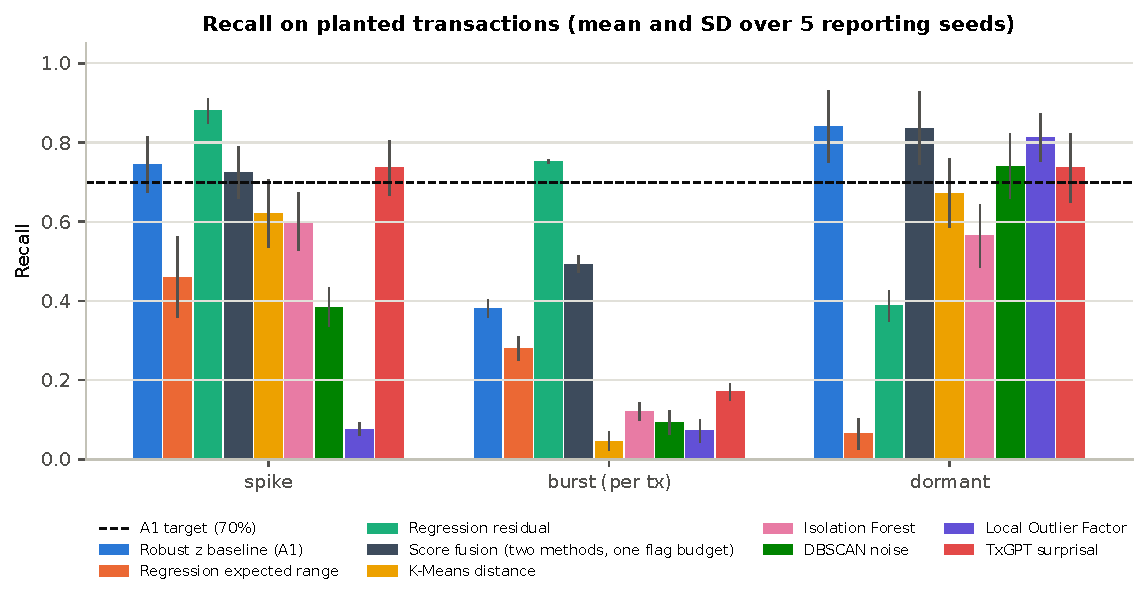
\includegraphics[width=0.8\textwidth]{eval_injection_recall.pdf}
\caption{Recall on planted transactions by pattern (mean and standard deviation over five reporting seeds). No
method is best at every pattern; the dashed line is Assignment~1's 70\% target.}
\label{fig:recall}
\end{figure}

\textbf{Regression and clustering} (Table~\ref{tab:unsupervised}). The random forest cuts the naive forecast's
error by \V{reg.gap_skill} on gaps but only \V{reg.size_skill} on amounts. Conformal calibration lifts the amount
range's coverage from \V{conf.before} to \V{conf.after} against a nominal \V{conf.nominal}, still slightly short.

\begin{table}[htbp]
\centering
\footnotesize
\caption{Regression and clustering metrics on DS1.}
\label{tab:unsupervised}
\begin{tabularx}{\textwidth}{@{}l Y r r r r@{}}
\toprule
Target & Model & MAE & RMSE & $R^2$ & Skill \\
\midrule
Amount & Naive forecast & 0.186 & 0.416 & 0.730 & 0.000 \\
Amount & Ridge & 0.181 & 0.373 & 0.783 & 0.027 \\
Amount & Random forest & 0.168 & 0.368 & 0.788 & 0.099 \\
Amount & Hist.\ gradient boosting & 0.189 & 0.389 & 0.764 & $-$0.015 \\
Gap & Naive forecast & 0.476 & 0.665 & 0.039 & 0.000 \\
Gap & Ridge & 0.279 & 0.410 & 0.635 & 0.414 \\
Gap & Random forest & 0.189 & 0.301 & 0.803 & 0.603 \\
Gap & Hist.\ gradient boosting & 0.192 & 0.298 & 0.807 & 0.597 \\
\bottomrule
\end{tabularx}
\par\smallskip\parbox{\textwidth}{\footnotesize Regression on the evaluation period, log10 scale; skill is 1 $-$ MAE / the naive forecast's MAE. Clustering, first search before the stages: K-Means $k=2$, silhouette 0.657, Davies--Bouldin 0.834; DBSCAN radius 1.3$\times$ the k-distance elbow, silhouette 0.786 without noise points, 2.0\% noise.}
\end{table}


\textbf{Agreement and stability over time.} The methods flag different transactions: the baseline's overlap
(Jaccard) with the other single methods is only \V{agree.base_range}, and \V{agree.base_txgpt} with TxGPT. Refitting
at \V{wf.cutoffs} walk-forward cut-offs keeps the baseline's mean recall at \V{wf.baseline_range}, so its result
does not depend on one split; LOF varies more (\V{wf.lof_range}).

\textbf{Unseen addresses: DS2 and DS10.} The frozen methods were tested on \V{ds2.check_addresses} DS2
histories and once on DS10 (Figure~\ref{fig:ds10}). Two outcomes were unexpected. First, methods tuned on DS1 fall
the most: fusion drops from \V{ds1.fusion.mean} to \V{ds10.fusion.mean} on DS10, below the baseline's
\V{ds10.baseline.mean}. Second, TxGPT, which learned from other addresses, ranks first on DS10
(\V{ds10.txgpt.mean}, interval \V{ds10.txgpt.ci}). Over 100 plant seeds the baseline ranks first among the
pooled methods on DS10 in \V{stats.ds10_baseline_rank1} of seeds. Bursts are hard to find on DS10, whose addresses
are busier and less regular (median gap \V{act.ds10_gap} hours against \V{act.ds1_gap} on DS1).

\begin{figure}[ht]
\centering
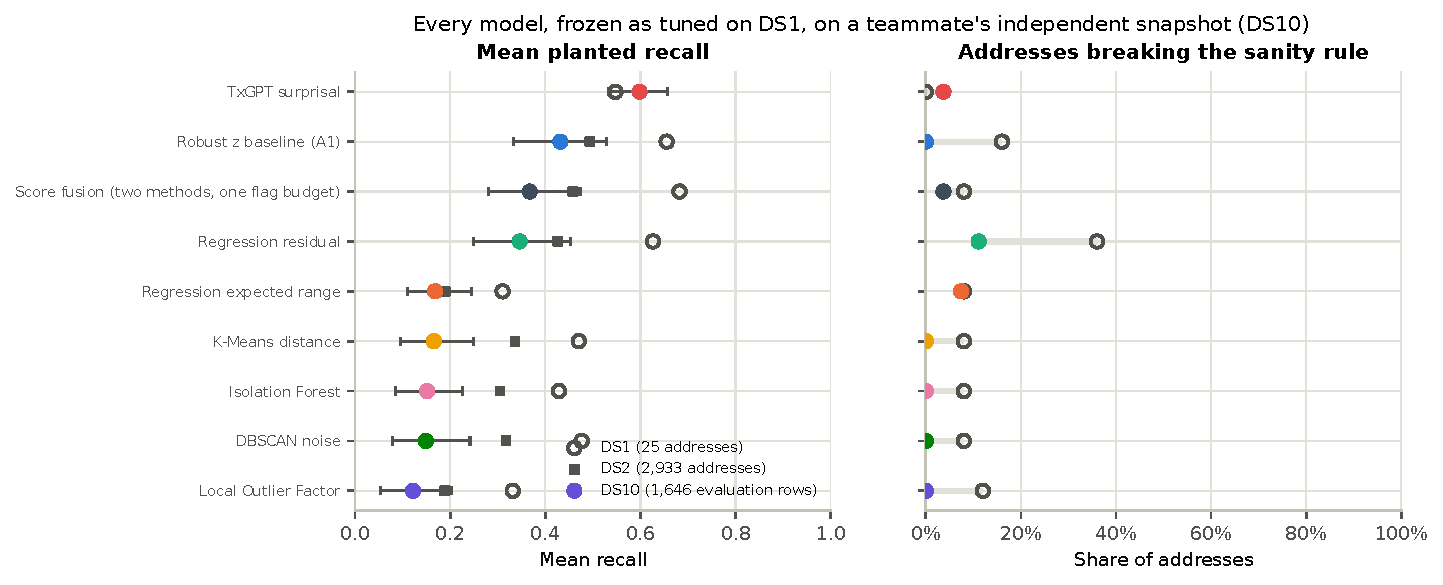
\includegraphics[width=0.95\textwidth]{eval_ds10_check.pdf}
\caption{Every method, frozen as tuned on DS1, on DS2 and the held-out DS10 (left: mean planted recall with
95\% bootstrap intervals on DS10; right: share of addresses breaking the sanity rule).}
\label{fig:ds10}
\end{figure}

\textbf{Classifiers on labelled data} (Table~\ref{tab:classifiers}). On Elliptic the random forest has the best
F1 (\V{cls.ell_rf_f1}, interval \V{cls.ell_rf_f1_ci} over ten training seeds), but every model collapses from
time step 43 (Figure~\ref{fig:elliptic}, Appendix~\ref{app:figures}), when a dark market closed and illicit behaviour changed (Pareja et al.\
2020). On BitcoinHeist's temporal split no model's F1 exceeds \V{cls.heist_temporal_max_f1}, and families held out of
training are found at recalls of \V{cls.lofo_range} by the tree models, consistent with Finding~4.

\begin{table}[htbp]
\centering
\footnotesize
\caption{Classifiers on the labelled datasets.}
\label{tab:classifiers}
\begin{tabularx}{\textwidth}{@{}L{3.6cm} Y r r r r r@{}}
\toprule
Data and split & Model & Accuracy & Precision & Recall & F1 & PR-AUC \\
\midrule
Elliptic, all features & Hist.\ gradient boosting & 0.971 & 0.808 & 0.734 & 0.769 & 0.803 \\
Elliptic, all features & k-nearest neighbours & 0.957 & 0.684 & 0.620 & 0.650 & 0.659 \\
Elliptic, all features & Logistic regression & 0.949 & 0.619 & 0.578 & 0.598 & 0.412 \\
Elliptic, all features & Random forest & 0.979 & 0.928 & 0.727 & 0.815 & 0.792 \\
Elliptic, local features & Hist.\ gradient boosting & 0.965 & 0.738 & 0.721 & 0.730 & 0.784 \\
Elliptic, local features & k-nearest neighbours & 0.969 & 0.792 & 0.703 & 0.745 & 0.741 \\
Elliptic, local features & Logistic regression & 0.969 & 0.839 & 0.640 & 0.726 & 0.619 \\
Elliptic, local features & Random forest & 0.970 & 0.801 & 0.721 & 0.759 & 0.781 \\
BitcoinHeist, temporal & Hist.\ gradient boosting & 0.705 & 0.012 & 0.722 & 0.024 & 0.042 \\
BitcoinHeist, temporal & k-nearest neighbours & 0.789 & 0.011 & 0.452 & 0.021 & 0.025 \\
BitcoinHeist, temporal & Logistic regression & 0.170 & 0.006 & 0.976 & 0.012 & 0.005 \\
BitcoinHeist, temporal & Random forest & 0.942 & 0.038 & 0.436 & 0.070 & 0.052 \\
BitcoinHeist, random & Hist.\ gradient boosting & 0.975 & 0.199 & 0.252 & 0.222 & 0.151 \\
BitcoinHeist, random & k-nearest neighbours & 0.957 & 0.099 & 0.254 & 0.143 & 0.071 \\
BitcoinHeist, random & Logistic regression & 0.510 & 0.020 & 0.691 & 0.039 & 0.017 \\
BitcoinHeist, random & Random forest & 0.979 & 0.250 & 0.239 & 0.244 & 0.177 \\
\bottomrule
\end{tabularx}
\par\smallskip\parbox{\textwidth}{\footnotesize Test splits: Elliptic time steps 35--49; BitcoinHeist years after the training years (temporal) or a random 20\%. Metrics are for the datasets' own positive classes (illicit; ransomware), at the threshold chosen on validation data.}
\end{table}


\textbf{Unusual is not a label.} Scored against the labelled classes, the unsupervised methods do worse than chance
(PR-AUC below the class share), while the random forest reaches \V{label.ell_rf_lift}$\times$ chance on Elliptic
(Appendix~\ref{app:figures}). Being unusual and belonging to a labelled class are different things, which supports
the Explorer's wording.

\textbf{Language models.} The Assistant passes the guardrail on \V{lm.guard_ds7} of DS7 test prompts and
\V{lm.guard_ds10} of DS10 prompts, and is fully correct (right reasons, order and numbers) on \V{lm.full_ds7} and
\V{lm.full_ds10}; pooled over twelve test sets, \V{lm.pooled} (\V{lm.pooled_ci}). Its weakest area is open glossary
questions, where it states \V{lm.glossary} of the key facts.

\textbf{Limitations.} Plants are our guess at what unusual looks like; DS1 has only 28 addresses, so intervals are
wide; methods tuned on DS1 transfer less well; and a language model can still give a wrong reason the guardrail
misses, so the template remains the default.

\FloatBarrier
\section{Conclusion}
\label{sec:conclusion}

We built and evaluated a pipeline that ranks an address's transactions by how unusual each is for that address.
Our answers:
\begin{enumerate}[label=RQ\arabic*]
  \item The baseline is the Explorer's method: within the margin of the best method on DS1, stable, explainable,
    and the most consistent on unseen addresses.
  \item Classifiers do well on Elliptic until behaviour changes, and stay weak on BitcoinHeist.
  \item Unusual activity and the labelled illicit class barely overlap: a flag is a reason to look, not a verdict.
  \item TxGPT, trained only on other addresses, ranks first on the held-out DS10; the Assistant explains
    flags faithfully under a guardrail, though it is weak on open questions.
\end{enumerate}

The main insight is that methods tuned on one sample of addresses lose much of their advantage on another, so an
independent held-out test was essential. Future work for Assignment~3 includes a web dashboard on the
prediction interface, live block data, TxGPT's surprisal beside the baseline, explanations refined from user
feedback, and a usability study with the intended users.


% Not counted: bibliography and appendix.
% Harvard (author-date in the text), numbered alphabetically as in Assignment 1. Every entry was verified on
% 29 Oct 2026 against Crossref, the publisher, arXiv or Zenodo (docs/REFERENCES.md). tools/report_build.py checks
% that every citation in the body has an entry here and every entry is cited.
\clearpage
\section*{References}
\addcontentsline{toc}{section}{References}

\begin{references}
\item Akcora, C.G., Li, Y., Gel, Y.R. and Kantarcioglu, M. (2020) `BitcoinHeist: topological data analysis for
  ransomware prediction on the Bitcoin blockchain', in \emph{Proceedings of the Twenty-Ninth International Joint
  Conference on Artificial Intelligence (IJCAI-20)}, pp.\ 4439--4445. doi: 10.24963/ijcai.2020/612.
\item Angelopoulos, A.N. and Bates, S. (2023) `Conformal prediction: a gentle introduction', \emph{Foundations and
  Trends in Machine Learning}, 16(4), pp.\ 494--591. doi: 10.1561/2200000101.
\item Ansel, J. et al.\ (2024) `PyTorch 2: faster machine learning through dynamic Python bytecode transformation
  and graph compilation', in \emph{Proceedings of the 29th ACM International Conference on Architectural Support
  for Programming Languages and Operating Systems, Volume 2 (ASPLOS '24)}, pp.\ 929--947.
  doi: 10.1145/3620665.3640366.
\item Ben Allal, L. et al.\ (2025) `SmolLM2: when smol goes big --- data-centric training of a small language
  model', \emph{arXiv preprint}, arXiv:2502.02737.
\item Blázquez-García, A., Conde, A., Mori, U. and Lozano, J.A. (2022) `A review on outlier/anomaly detection in
  time series data', \emph{ACM Computing Surveys}, 54(3), pp.\ 1--33. doi: 10.1145/3444690.
\item Blockstream (n.d.) \emph{Esplora HTTP API}. Available at:
  \url{https://github.com/Blockstream/esplora/blob/master/API.md} (Accessed: 22 October 2026).
\item Boukerche, A., Zheng, L. and Alfandi, O. (2021) `Outlier detection: methods, models, and classification',
  \emph{ACM Computing Surveys}, 53(3), pp.\ 1--37. doi: 10.1145/3381028.
\item Bushra, A.A. and Yi, G. (2021) `Comparative analysis review of pioneering DBSCAN and successive
  density-based clustering algorithms', \emph{IEEE Access}, 9, pp.\ 87918--87935.
  doi: 10.1109/ACCESS.2021.3089036.
\item Chicco, D. and Jurman, G. (2020) `The advantages of the Matthews correlation coefficient (MCC) over F1 score
  and accuracy in binary classification evaluation', \emph{BMC Genomics}, 21, 6. doi: 10.1186/s12864-019-6413-7.
\item Elmougy, Y. and Liu, L. (2023) `Demystifying fraudulent transactions and illicit nodes in the Bitcoin
  network for financial forensics', in \emph{Proceedings of the 29th ACM SIGKDD Conference on Knowledge Discovery
  and Data Mining (KDD '23)}, pp.\ 3979--3990. doi: 10.1145/3580305.3599803.
\item Grinsztajn, L., Oyallon, E. and Varoquaux, G. (2022) `Why do tree-based models still outperform deep
  learning on typical tabular data?', \emph{Advances in Neural Information Processing Systems}, 35, Datasets and
  Benchmarks Track. arXiv:2207.08815.
\item Han, S., Hu, X., Huang, H., Jiang, M. and Zhao, Y. (2022) `ADBench: anomaly detection benchmark',
  \emph{Advances in Neural Information Processing Systems}, 35, Datasets and Benchmarks Track. arXiv:2206.09426.
\item Hilal, W., Gadsden, S.A. and Yawney, J. (2022) `Financial fraud: a review of anomaly detection techniques
  and recent advances', \emph{Expert Systems with Applications}, 193, 116429. doi: 10.1016/j.eswa.2021.116429.
\item Hoffmann, J. et al.\ (2022) `An empirical analysis of compute-optimal large language model training',
  \emph{Advances in Neural Information Processing Systems}, 35. arXiv:2203.15556.
\item Ikotun, A.M., Ezugwu, A.E., Abualigah, L., Abuhaija, B. and Heming, J. (2023) `K-means clustering
  algorithms: a comprehensive review, variants analysis, and advances in the era of big data',
  \emph{Information Sciences}, 622, pp.\ 178--210. doi: 10.1016/j.ins.2022.11.139.
\item Ji, Z. et al.\ (2023) `Survey of hallucination in natural language generation', \emph{ACM Computing
  Surveys}, 55(12), pp.\ 1--38. doi: 10.1145/3571730.
\item Kapoor, S. and Narayanan, A. (2023) `Leakage and the reproducibility crisis in machine-learning-based
  science', \emph{Patterns}, 4(9), 100804. doi: 10.1016/j.patter.2023.100804.
\item Lai, K.-H., Zha, D., Xu, J., Zhao, Y., Wang, G. and Hu, X. (2021) `Revisiting time series outlier
  detection: definitions and benchmarks', \emph{Proceedings of the Neural Information Processing Systems Track on
  Datasets and Benchmarks}, 1 (NeurIPS 2021). Available at:
  \url{https://datasets-benchmarks-proceedings.neurips.cc/paper/2021/hash/ec5decca5ed3d6b8079e2e7e7bacc9f2-Abstract-round1.html}
  (Accessed: 29 October 2026).
\item Le, V.-H. and Zhang, H. (2022) `Log-based anomaly detection with deep learning: how far are we?', in
  \emph{Proceedings of the 44th International Conference on Software Engineering (ICSE '22)}, pp.\ 1356--1367.
  doi: 10.1145/3510003.3510155.
\item mempool.space (n.d.) \emph{REST API documentation}. Available at: \url{https://mempool.space/docs/api/rest}
  (Accessed: 22 October 2026).
\item Pareja, A. et al.\ (2020) `EvolveGCN: evolving graph convolutional networks for dynamic graphs',
  \emph{Proceedings of the AAAI Conference on Artificial Intelligence}, 34(04), pp.\ 5363--5370.
  doi: 10.1609/aaai.v34i04.5984.
\item Penedo, G. et al.\ (2024) `The FineWeb datasets: decanting the web for the finest text data at scale',
  \emph{Advances in Neural Information Processing Systems}, 37, pp.\ 30811--30849. doi: 10.52202/079017-0970.
\item Pineau, J. et al.\ (2021) `Improving reproducibility in machine learning research (a report from the
  NeurIPS 2019 reproducibility program)', \emph{Journal of Machine Learning Research}, 22(164), pp.\ 1--20.
\item scikit-learn developers (2025) \emph{scikit-learn} (Version 1.6.1) [Software]. Zenodo.
  doi: 10.5281/zenodo.14627164.
\item The Matplotlib Development Team (2025) \emph{Matplotlib: visualization with Python} (Version 3.10.1)
  [Software]. Zenodo. doi: 10.5281/zenodo.14940554.
\item The pandas development team (2024) \emph{pandas-dev/pandas: Pandas} (Version 2.2.3) [Software]. Zenodo.
  doi: 10.5281/zenodo.13819579.
\item Touvron, H. et al.\ (2023) `LLaMA: open and efficient foundation language models', \emph{arXiv preprint},
  arXiv:2302.13971.
\item UCI Machine Learning Repository (2020) \emph{Bitcoin Heist Ransomware Address} [Dataset].
  doi: 10.24432/C5BG8V. Available at:
  \url{https://archive.ics.uci.edu/dataset/526/bitcoinheistransomwareaddressdataset} (Accessed: 20 October 2026).
\end{references}

\appendix
% Appendix (not counted towards the word limit).
\clearpage
\section{Example prediction}
\label{app:example}

The output below is what Assignment~3's back end receives. It was produced by
\code{python -m explorer.cli predict what-if} on a hypothetical transaction of one DS1 address: sending
0.05~BTC, about a hundred times the address's usual amount. The size features (F1, F4) pass the flag line;
the timing features (F2, F3) are within the usual range, so they are not mentioned.

{\footnotesize
\begin{verbatim}
input:    0.05 BTC out at 2026-10-20T12:00Z, address 1Bbcsfxj2JRUD5crcdZVHBcViT61vrJ3dz
scored: true   flagged: true   score (largest |z|): 5.98
feature                     value        usual       z  role
F1 Size                      0.05  0.000524948    5.88  flag
F2 Burst                        3            4   -0.45  within-usual
F3 Gap                    21.8264      10.0535    0.30  within-usual
F4 Relative size          95.2472     0.909938    5.98  flag
\end{verbatim}
}
Explanation shown to the user (template writer):
{\footnotesize
\begin{verbatim}
Flagged by Robust z baseline (A1).
What stands out compared with this address's own history:
- Higher ratio to the usual amount than usual: 95.2x the usual amount for this direction, against a
  usual 0.9x.
- Larger amount than usual: 0.05 BTC moved, against a usual 0.00052495 BTC.
Unusual activity requires investigation; it does not indicate wrongdoing.
\end{verbatim}
}


\section{Further results}
\label{app:figures}

\begin{figure}[H]
\centering
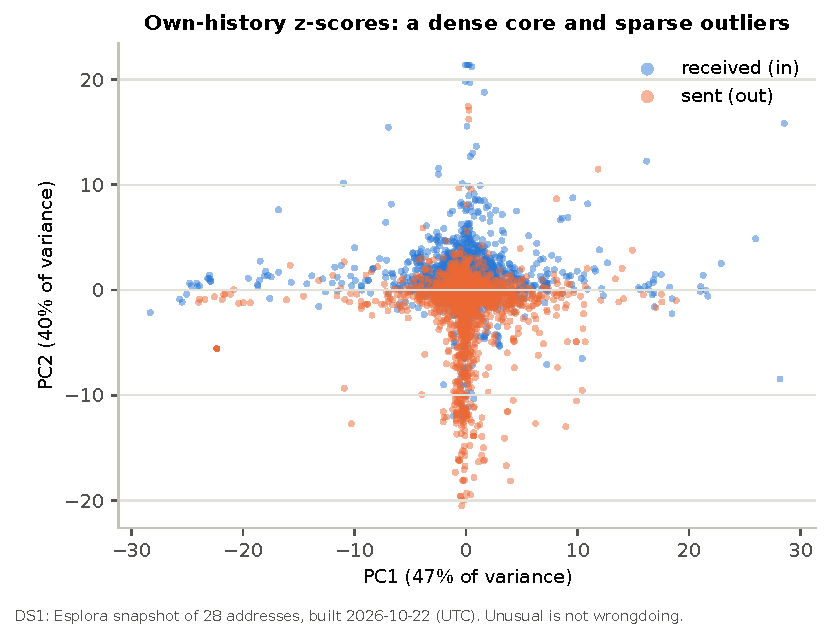
\includegraphics[width=0.78\textwidth]{eda_pca.pdf}
\caption{DS1's transactions on the first two principal components, showing a dense core with sparse outliers
(Finding~3).}
\label{fig:pca}
\end{figure}

\begin{figure}[H]
\centering
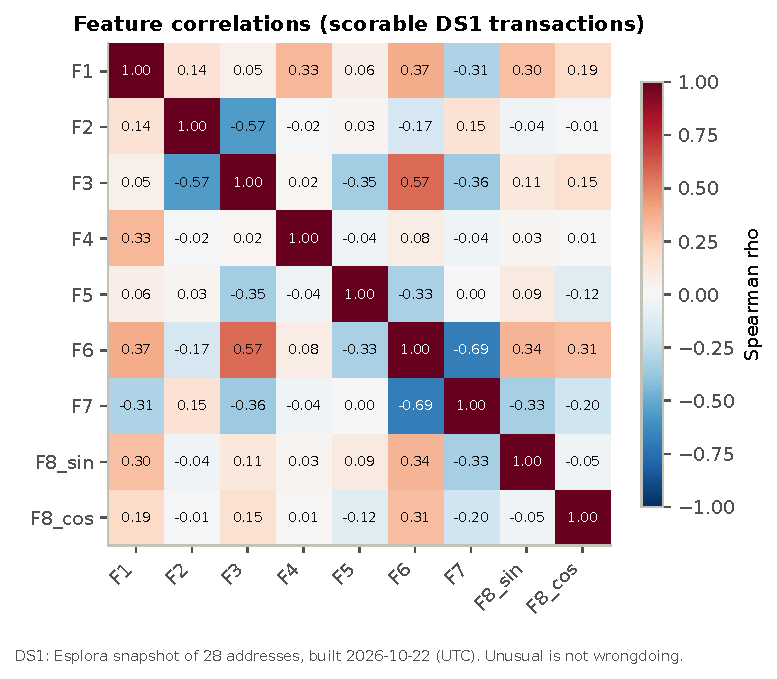
\includegraphics[width=0.72\textwidth]{eda_feature_correlation.pdf}
\caption{Rank correlations between DS1's features (Finding~3).}
\label{fig:correlation}
\end{figure}

\begin{figure}[H]
\centering
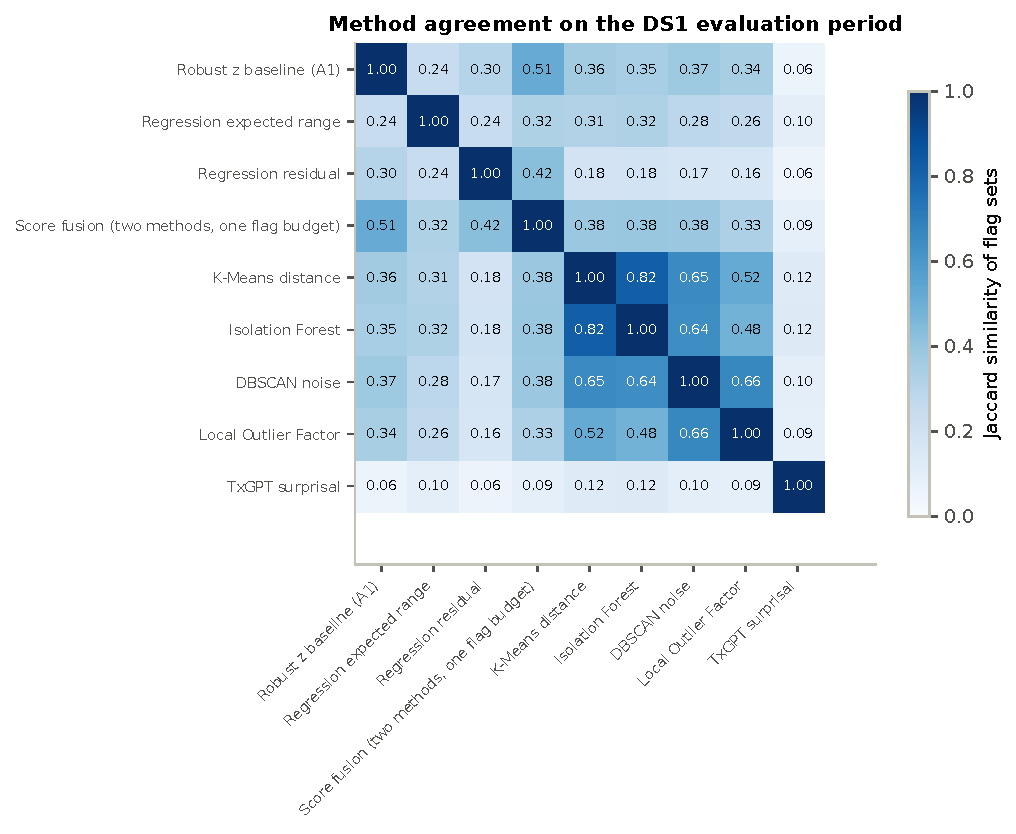
\includegraphics[width=0.78\textwidth]{eval_agreement.pdf}
\caption{Pairwise Jaccard overlap between the methods' flagged transactions (\code{eval\_agreement.csv}).}
\label{fig:agreement}
\end{figure}

\begin{figure}[H]
\centering
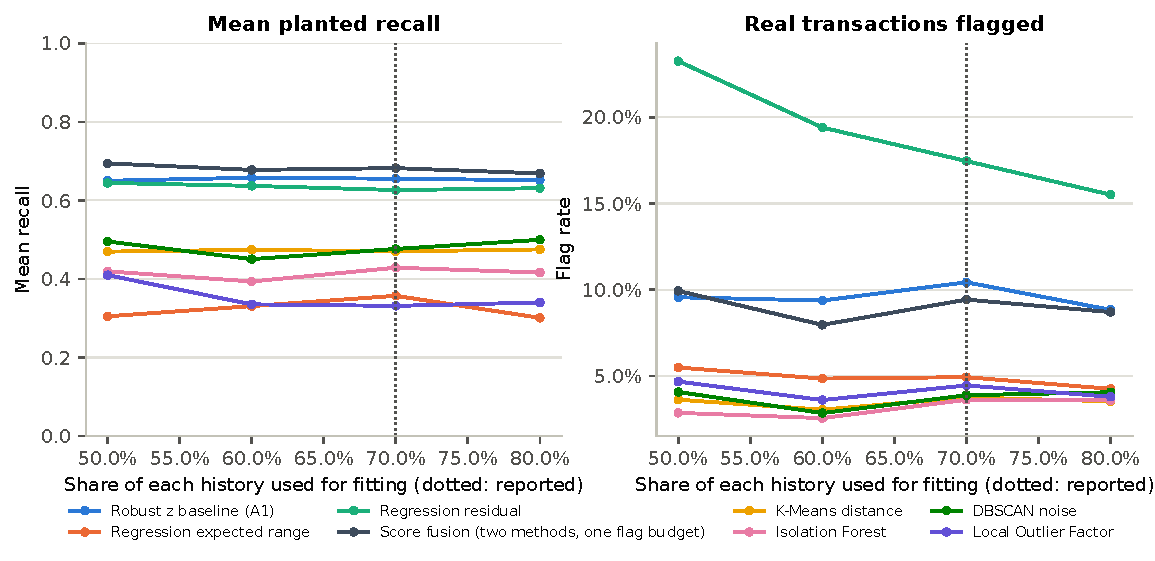
\includegraphics[width=0.85\textwidth]{eval_walkforward.pdf}
\caption{Every method refitted at each walk-forward cut-off (\code{eval\_walkforward.csv}).}
\label{fig:walkforward}
\end{figure}

\begin{figure}[H]
\centering
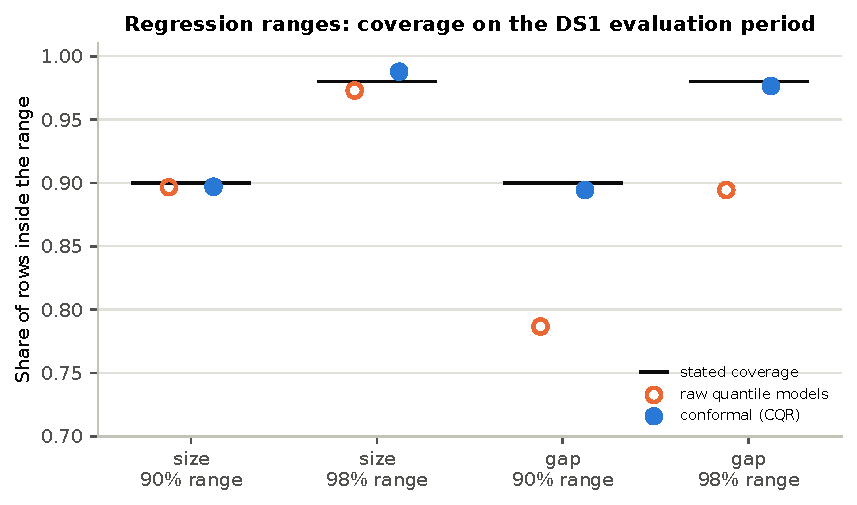
\includegraphics[width=0.8\textwidth]{eval_conformal.pdf}
\caption{Coverage of the regression ranges before and after conformal calibration
(\code{regression\_results.csv}).}
\label{fig:conformal}
\end{figure}

\begin{figure}[H]
\centering
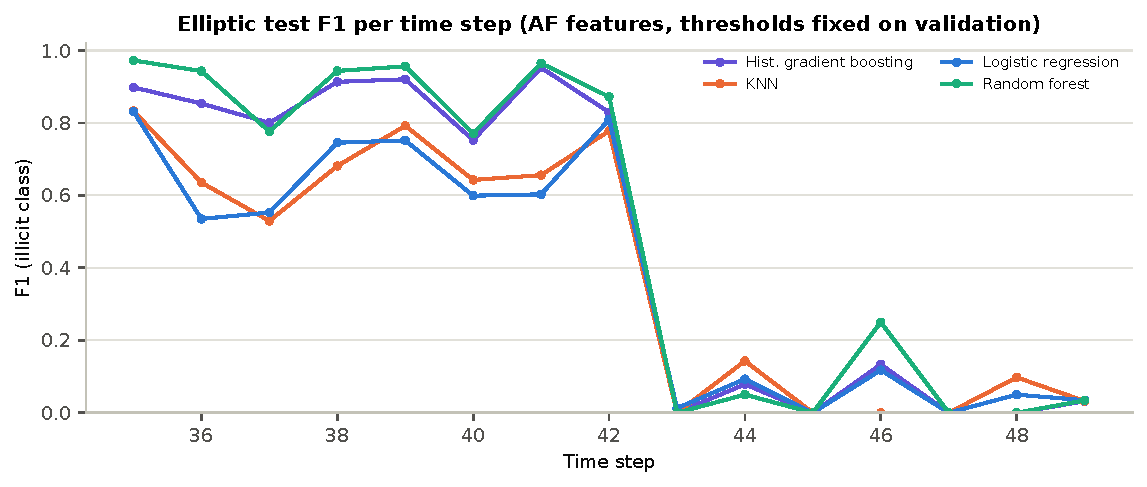
\includegraphics[width=0.82\textwidth]{eval_elliptic_f1_by_step.pdf}
\caption{Elliptic test F1 per time step. Every model fails from step 43, after the shutdown of a dark market
changed the illicit class's behaviour.}
\label{fig:elliptic}
\end{figure}

\begin{figure}[H]
\centering
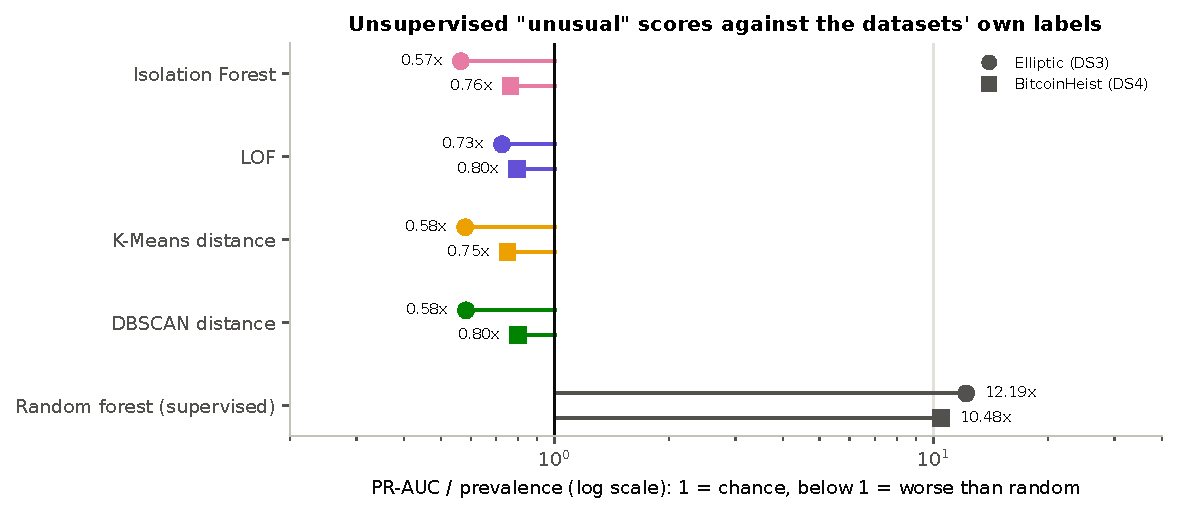
\includegraphics[width=0.9\textwidth]{eval_label_check.pdf}
\caption{Unsupervised scores against the labelled datasets' own classes. Every unsupervised method is below
chance (1$\times$), while the supervised random forest is far above it: being unusual is not the same as
belonging to a labelled class (\code{label\_check.csv}).}
\label{fig:labelcheck}
\end{figure}

\begin{figure}[H]
\centering
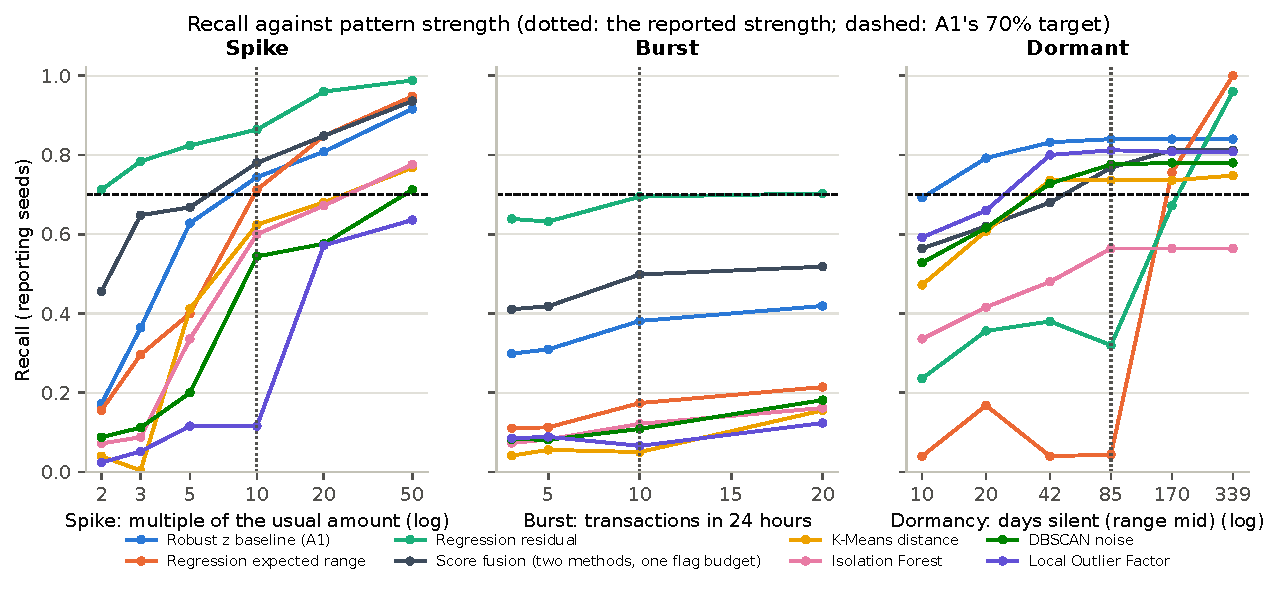
\includegraphics[width=0.9\textwidth]{eval_sensitivity.pdf}
\caption{Recall against the strength of each planted pattern (\code{eval\_sensitivity.csv}). Weaker plants are
harder for every method; regression keeps finding small spikes that the baseline misses.}
\label{fig:sensitivity}
\end{figure}

\begin{figure}[H]
\centering
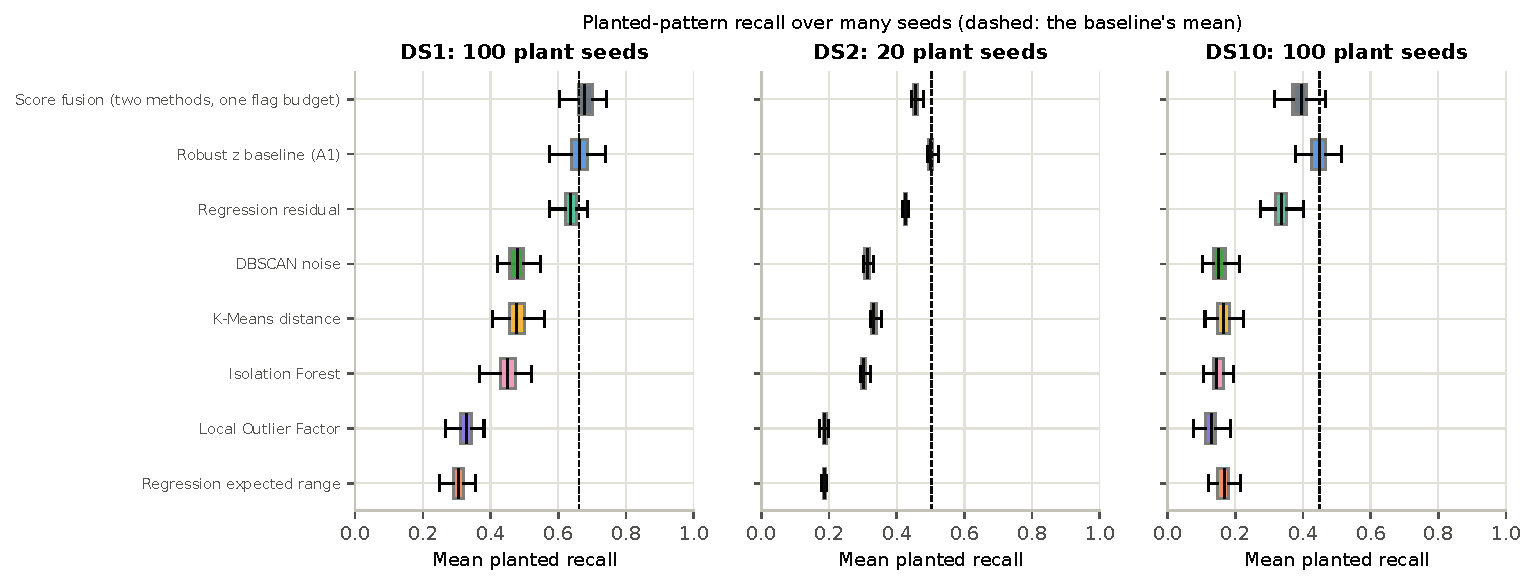
\includegraphics[width=0.9\textwidth]{stats_methods.pdf}
\caption{Mean planted recall over 100 plant seeds on DS1 and DS10 and 20 on DS2
(\code{stats\_methods\_summary.csv}).}
\label{fig:statsmethods}
\end{figure}

\begin{figure}[H]
\centering
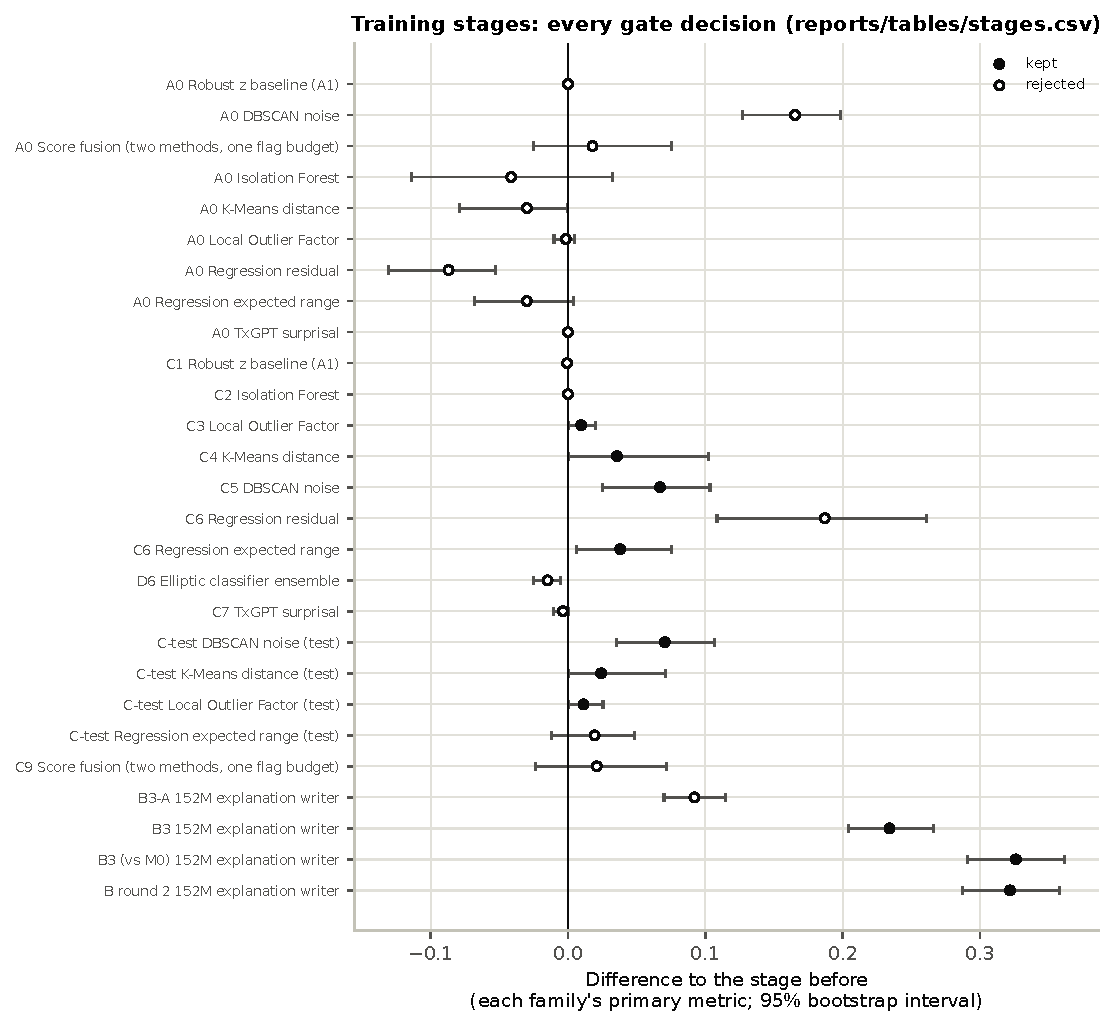
\includegraphics[width=0.9\textwidth]{eval_stages.pdf}
\caption{Every training stage's gate decision with its bootstrap interval (\code{stages.csv}).}
\label{fig:stages}
\end{figure}

\begin{figure}[H]
\centering
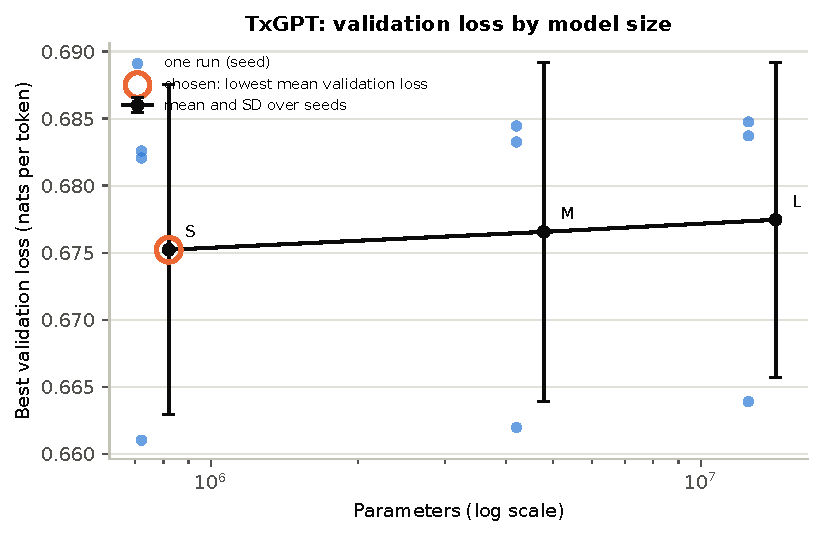
\includegraphics[width=0.75\textwidth]{eval_txgpt_sizes.pdf}
\caption{TxGPT's validation loss for three sizes and three seeds each (\code{txgpt\_sizes.csv}). The sizes tie,
so the smallest was kept.}
\label{fig:txgpt}
\end{figure}

\begin{figure}[H]
\centering
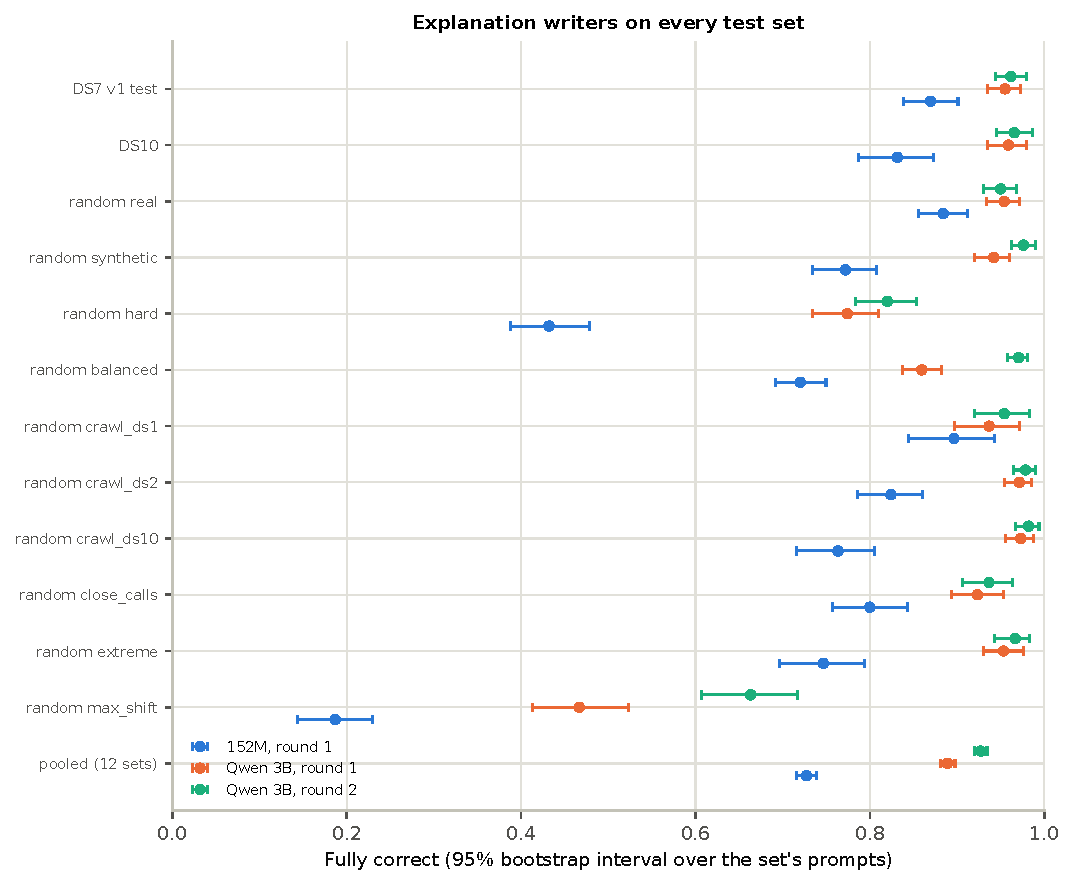
\includegraphics[width=0.9\textwidth]{stats_writers.pdf}
\caption{The Assistant's fully correct rate on each test set, before (round 1) and after (round 2) its second
training round, with 95\% bootstrap intervals (\code{stats\_writers\_summary.csv}).}
\label{fig:writers}
\end{figure}

\section{Reproducing the results}
\label{app:repro}

The repository's \code{README.md} gives every command. In short:
\begin{verbatim}
conda env create -f environment.yml
conda activate cos30049-a2
python -m pytest -q                     # the test suite
python -m explorer.cli all --offline    # every DS1 result
python -m explorer.cli figures
python tools/compare_tables.py          # rebuild against the committed tables
\end{verbatim}
\code{DATA\_CARD.md} documents every dataset, file and column, and \code{MODEL\_CARD.md} every final model.


\end{document}
